\documentclass[11pt,a4paper]{article}
\usepackage[utf8]{inputenc}
\usepackage[german]{babel}
\usepackage{amsmath}
\usepackage{amsfonts}
\usepackage[urlcolor=blue]{hyperref}
\usepackage{booktabs}
\usepackage{setspace}
\usepackage{threeparttable}
\usepackage{amssymb}
\usepackage{graphicx}
\usepackage{fancyhdr}
\usepackage{icomma}
\usepackage{float}
\usepackage{pdfpages}
\usepackage[left=2.5cm,right=2.5cm,top=2cm,bottom=3.5cm]{geometry}
\usepackage{csquotes}
\usepackage{chngcntr}	% Damit Listings Listing 1.1 etc heißen
\usepackage{minted}
\usepackage{xcolor,soul,lipsum}
\renewcommand\listoflistingscaption{Listings}

\counterwithin{listing}{section} % Korrektes Counting

\title{WeatherWallpaper\vspace{20px}}
\author{Janis Fix, Leon Gieringer \\ \\ TINF18B3 \\ \\ \\ Advanced Software Engineering \\ \\ \\ \\}
\date{\today}

\begin{document}
	\maketitle
	\thispagestyle{empty}
	\newpage
	
	\pagenumbering{Roman}
	\tableofcontents
	\newpage
	\listoflistings
	\newpage
	
	%\listoffigures
	%\newpage
	
	\pagenumbering{arabic}
	\pagestyle{fancy}
	\fancyhf{}
	\setlength{\headheight}{35pt}
	\lhead{WeatherWallpaper}
	\rhead{Advanced Software Engineering}
	\cfoot{\thepage}
	\newpage
	
	
	\section{Einleitung}
	Hier steht meine Einleitung
	\clearpage
	
	\section{Clean Architecture}
	Softwareprodukte entwickeln sich immer weiter, was heute noch State of the art ist, kann in ein paar Jahren schon wieder durch eine neue Technologie ersetzt worden sein. Deshalb ist es wichtig seine Anwendung so gut wie möglich für Technologie-Änderungen von außen vorzubereiten. Um dies zu ermöglichen, muss bei den Architekturentscheidung acht gegeben werden. Dabei sollte man sich nicht an äußere Abhängigkeiten binden, sondern diese austauschbar machen. Dabei teilt sich der Quellcode einer Anwendung in mindestens zwei Schichten ein. Der langfristig bestehende Quellcode der Anwendung, sowie der kurzlebige Quellcode der äußeren Abhängigkeiten. Zu diesen äußeren Abhängigkeiten kann beispielsweise eine API gehören. Dieser Schichtenaufbau ist vergleichbar mit einer Matrjoschka oder einer Zwiebel.\\

\noindent Wie bei einer Matrjoschka/Zwiebel auch, muss die Dependency Rule erfüllt sein, damit die Schichten klar aufgeteilt sind und äußere Schichten (relativ) einfach ausgetauscht werden können. Die Dependecy Rule sagt aus, dass Abhängigkeiten immer nur von außen nach innen gehen dürfen. Wenn ein äußerer Zwiebelring ausgetauscht wird, soll dies keine Änderung bzw. Anpassung an einem weiter innen liegenden Zwiebelring bewirken.\\

\noindent Eine Applikation lässt sich in fünf Schichten einteilen, das sind (von innen nach außen):\\

\noindent
\hangindent1cm
\textbf{Der Abstraction Code}
Dieser beinhaltet Code, der sowohl für die eigene Problemdomäne, als auch andere Problemdomänen wichtig sein kann. Hierzu zählen beispielsweise mathematische Grundlagen, wie Vektoren o.Ä.\\

\noindent
\hangindent1cm
\textbf{Der Domain Code}
Diese Schicht beinhaltet hauptsächlich Entitäten und sollte sich am wenigsten ändern.\\

\noindent
\hangindent1cm
\textbf{Der Application Code}
Im Application Code sind die einzelnen Use Cases wieder zu finden und implementiert damit die Geschäftslogik der Anwendung. Hier werden also die einzelnen Use Cases umgesetzt.\\

\noindent
\hangindent1cm
\textbf{Die Adapter}
Diese Schicht handelt, wie der Name schon sagt, als Adapter zwischen den äußeren Plugins und den inneren Schichten. Dabei kann beispielsweise eine Formatkonvertierung stattfinden. Ein Beispiel hierfür wäre eine Web-API, die in der Plugin-Schicht angeordnet ist und ein JSON-String zurückliefert. Der Adapter ist dann für die Konvertierung des JSON-Objekts zu dem Format der Anwendung (z.B. C\#-Objekt) zuständig. Ziel der Adapter ist es, die inneren und äußeren Schichten zu entkoppeln.\\

\noindent
\hangindent1cm
\textbf{Die Plugins}
Diese Schicht darf keine Anwendungslogik enthalten, da die Plugins jederzeit änderbar sein müssen. Hier steht quasi nur Pure Fabrication Code. Wird beispielsweise das World-Wide-Web durch eine besondere neue Technologie ersetzt, müssen die Web-APIs ausgetauscht werden. Dies sollte sich nicht auf die anwendungsspezifische Geschäftslogik auswirken.\\

\noindent Die Applikation wird in einer vier Schichtenarchitektur umgesetzt. Dabei wird auf die erste Schicht, den Abstraction Code, verzichtet.
\subsection{Vorher}\label{CleanArchitectureVorher}
Ein UML-Diagramm mit der Situation vor dem Implementieren der Clean Architecture ist auf unserem Git-Repository \href{https://github.com/Bronzila/WeatherWallpaper/blob/master/CleanArchitecturePics/Architektur_Vorher.jpg}{\color{blue}hier} zu finden. Abhängigkeiten von innen nach außen, die die Dependecy Rule brechen, sind dick und rot hinterlegt. Auf die Abhängigkeitspfeile in die innerste Schicht wurde für die Leserlichkeit verzichtet.
\subsection{Nachher}
Neben der Implementierung der Clean Architecture wurden natürlich auch noch andere Än"-de"-rung"-en beispielsweise für die Programming Principles umgesetzt. Daher haben sich manche Klassen aufgeteilt. Das aktuelle UML-Diagramm der Anwendung findet man \href{https://github.com/Bronzila/WeatherWallpaper/blob/master/CleanArchitecturePics/UML_Aktuell.jpg}{\color{blue}hier}. Hierbei ist erkennbar, dass nun keine Abhängigkeitspfeile von einer inneren zu einer äußeren Schicht gehen und diese mithilfe der Dependency Inversion umgedreht wurden. Damit ist die Depedency Rule erfüllt. Im Folgenden wird nochmals genauer auf die einzelnen Schichten eingegangen.
\subsubsection{Domain Code}
In dieser Schicht reihen sich die Entitäten der Anwendung ein. Dazu gehört die \texttt{Config}, in der das Zeitintervall und der Standort gespeichert ist, sowie die \texttt{Weather}- und \texttt{ImageResponse}, welche die für die Anwendung nötigen Daten der APIs wiedergeben. In der Klasse \texttt{CountryArrays} sind Länder und ihre Abkürzungen hinterlegt. Die \texttt{WeatherInterpretation} wird für die Interpretierung des Wetters verwendet und die \texttt{BadConfigException} ist ein eigener Exception-Typ, der angibt, dass die Konfiguation fehlerhaft ist. Im UML-Diagramm wird erneut auf die Abhängigkeitspfeile in die innerste Schicht verzichtet, damit es lesbarer bleibt.
\subsubsection{Application Code}
Die zentrale Klasse der Anwendung und des Application Codes ist der \texttt{Refresher}. Mithilfe des Refreshers lässt sich, über Delegation an Helferklassen, das Desktophintergrundbild an die aktuelle Wettersituation anpassen. Dafür muss beispielsweise das aktuelle Wetter interpretiert werden, so dass man eine deskriptive Darstellung des Wetters zum Abfragen der Bild-API hat. Dies wird von der \texttt{WeatherInterpreter}-Klasse erledigt. Ein weiterer Use-Case ist die Validierung der vom Nutzer eingegebenen Konfiguration. Darum kümmert sich der \texttt{ConfigValidator}. Dafür arbeitet sie mit den \texttt{IValidationAspects} zusammen. Näheres dazu ist bei dem OCP beschrieben. Der \texttt{ConfigKeeper} verwaltet die aktuelle Konfiguration der Anwendung. Die Klassen \texttt{ScreenChangeWorker} und \texttt{UpdateTimer} werden für das aktualisieren mithilfe des Refreshers verwendet. Ersterer wird verwendet, um ein manuelles Aktualisieren in einem neuen Thread zu gewährleisten, damit die GUI nicht blockiert wird. Zweiterer ist für das zyklische Aktualisieren des Hintergrunds zuständig. In dieser Schicht sind ebenfalls die benötigten Interfaces für den Zugriff auf äußere Schichten vorhanden, so dass die Dependency Rule eingehalten wird.
\subsubsection{Adapters}
In der Adapter-Schicht sind sowohl die Adapter für die Wetter- und Bild-API, als auch für die Konfiguration vorhanden. In dem \texttt{Image-} und \texttt{WeatherHandler} werden die JSON-Objekte, die von der API kommen, zu C\#-Objekten gemapt und andersrum mithilfe einer Liste von strings die Routenparameter zusammengebaut und an die API weitergegeben. Der \texttt{ConfigHandler} wandelt die als JSON gespeicherte Konfigurationsdatei in ein C\#-Objekt um, damit diese geladen werden kann. In die andere Richtung wird zum Abspeichern der Konfiguration aus dem C\#-Objekt ein string gemacht. Eine weitere Klasse, die sich in die Adapter-Schicht einordnen lässt, ist der \texttt{MainWindowController}. Hierbei werden die Eingaben der GUI weiter gereicht. Ein Beispiel hierfür ist das manuelle Aktualisieren des Hintergrunds. Dabei gibt die GUI dieses Signal an den \texttt{MainWindowController} weiter, welcher dann mithilfe des \texttt{ScreenChangeWorkers} den Hintergrund aktualisiert.
\subsubsection{Plugins}
In der Plugin-Schicht ist der \texttt{APICaller} angesiedelt, der eine API aufrufen kann. Falls eine neue Technologie für die API entwickelt wird bzw. verwendet werden soll, muss nur der \texttt{APICaller} ausgetauscht/verändert werden. Das \texttt{ErrorModel} gehört eng zum \texttt{APICaller}, da bei einem fehlerhaften HTTP-Call in diesem Model der Statuscode gespeichert und an den Adapter zurückgegeben wird. Zur Plugin-Schicht gliedert sich auch der \texttt{DownloadHelper} ein, der ein Bild aus dem Internet herunter läd. Der \texttt{ImageWriter} kann ein Bild auf die Festplatte schreiben und der \texttt{FileAccessor} kann generell Dateien auf der Festplatte lesen und schreiben. Sollte sich das Dateisystem oder Speichermedium ändern, müsste der Code angepasst werden und ist dementsprechend in der äußersten Schicht. Auch der \texttt{BackgroundChanger} ordnet sich in er Plugin-Schicht ein, da dieser nur für das Windows-Betriebssystem den Hintergrund ändern kann. Möchte man das Betriebssystem ändern, so müsste auch er angepasst werden. Selbes gilt für den \texttt{StartupHelper}, der die Anwendung in den Autostart des Windows-Systems setzt bzw. von dort wieder entfernt. Zu guter Letzt ist die GUI Teil der Plugin-Schicht. Sollte in Zukunft beispielsweise auf eine Web-Oberfläche anstelle einer aktuellen WindowsForms-Oberfläche gewechselt werden, so müsste dieses Plugin angepasst werden.
\subsubsection{Mögliche Erweiterungen/Probleme}
Da beim Beginn des Projektes die API-Responses (\texttt{WeatherResponse} und \texttt{ImageResponse}) auch für die Verarbeitung im Code weiterverwendet wurden, sind sie aktuell als Entität im Domain-Code hinterlegt. Sollte sich nun allerdings das Format der API bzw. die API generell ändern, so müssten neue Klassen zum Mappen hinzugefügt werden. Diese neuen Klassen würden sich dann in der Adapter-Schicht befinden und der jeweilige Adapter (z.B. \texttt{WeatherHandler}) müsste dann erst das JSON-Objekt auf diese Klasse mappen. Nach dem Mapping schreibt der \texttt{WeatherHandler} dann die benötigten Informationen in das \texttt{WeatherResponse}-Objekt, damit dieses dann intern weiterverwendet werden kann.
	\clearpage
	\section{Entwurfsmuster}
	% TODO
\begin{itemize}
	\item $>= 1$ Entwurfsmuster einsetzen und begründen

	\item UML-Diagramm vorher und nachher
\end{itemize}
	\clearpage
	\section{Programming Principles}
	\subsection{SOLID}
\subsubsection{Single Responsibility Principle}
\label{sec:srp}
Das Single Responsibility Principle (SRP) wird auch als Prinzip der einzigen Zuständigkeit bezeichnet. Dementsprechend soll eine Klasse nur einen Grund haben, um geändert werden zu müssen. Dadurch erhält jedes Objekt eine klar definierte Aufgabe. Durch das Anwenden dieses Prinzips, wird die Seperation of Concerns (SoC) umgesetzt. Sollte das Prinzip der Single Responsibility verletzt sein, so lässt sich dies relativ einfach mit der Antwort auf die Frage \glqq{}Was macht die Klasse?\grqq{} herausfinden. Sollte sich eine Konjunktion in der Antwort auf diese Frage befinden, kann man davon ausgehen, dass das SRP verletzt ist.\\

\noindent Als Beispiel für die Anwendung des SRP wird der ehemalige \texttt{MainController} betrachtet. Die Klasse als UML ist in Abbildung \ref{MainController} zu sehen. Auf die Frage \glqq{}Was macht die Klasse?\grqq{} lassen sich vier Antworten finden:
\begin{itemize}
\item Die generelle Logik, um den Hintergrund zu aktualisieren.
\item Das Halten und Verwalten des Timers für die zyklische Aktualisierung des Hintergrundbilds.
\item Die Logik, um das Hintergrundbild manuell in einem neuen Thread zu aktualisieren.
\item Das Weitergeben einer neuen Config zum Speichern bzw. das Abrufen der aktuellen Config.
\end{itemize}

\begin{figure}[ht]
\centering
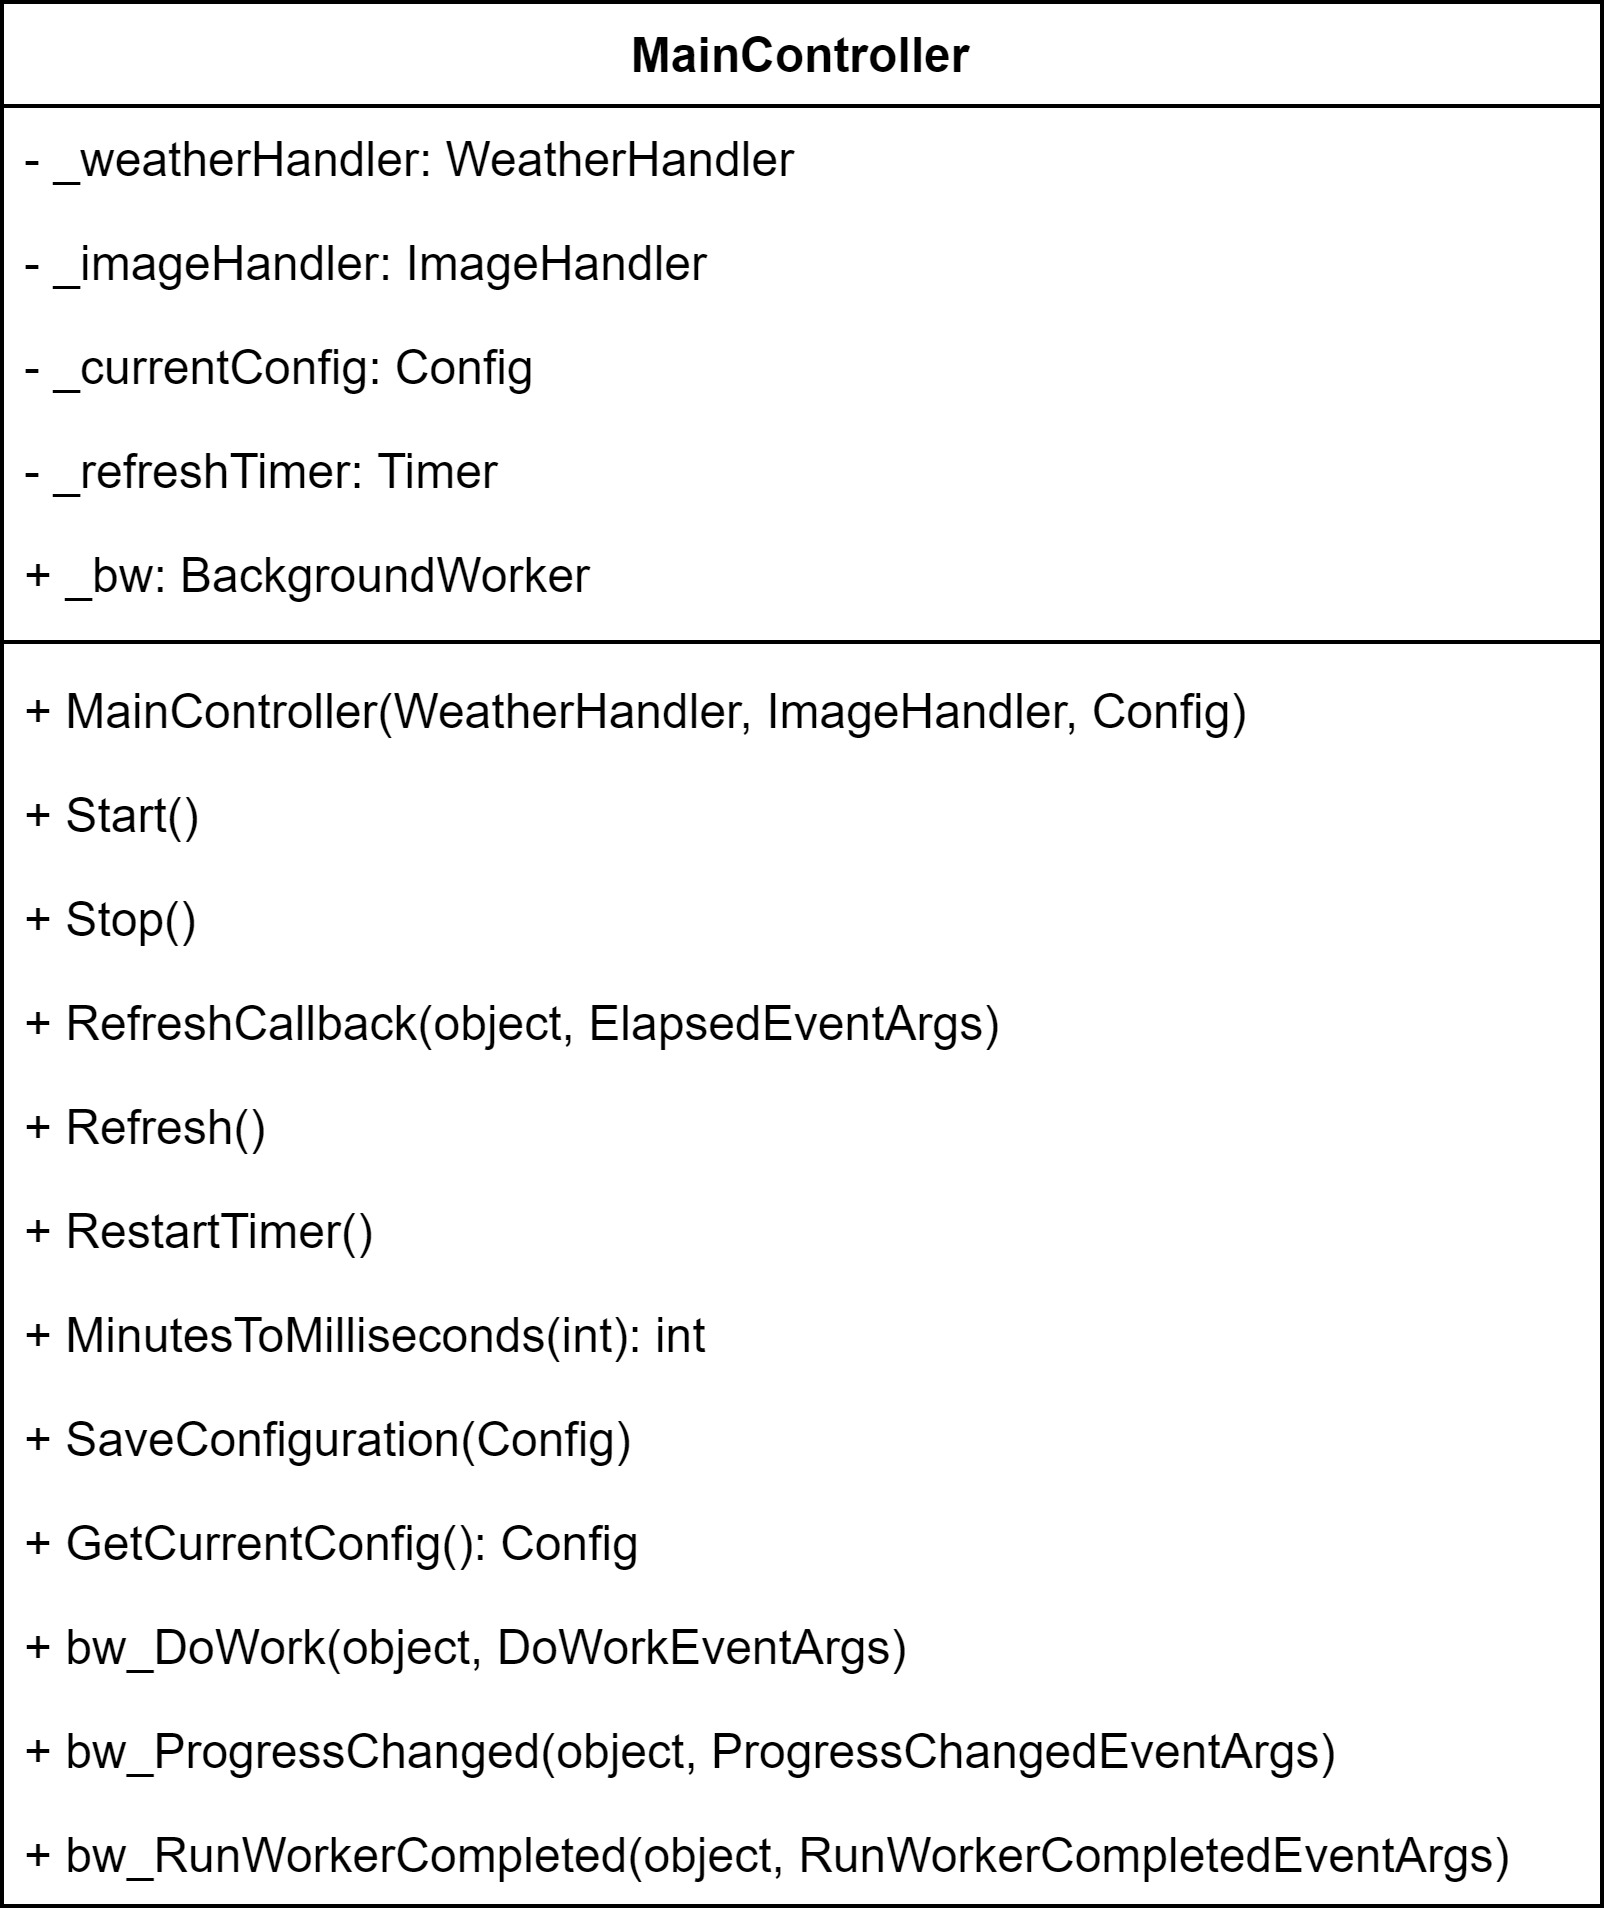
\includegraphics[width=0.5\textwidth]{Bilder/MainController}
\caption[MainController in UML-Form]{\label{MainController} MainController in UML-Form}
\end{figure}

\noindent Um diese verschiedenen Responsibilities in neue Klassen aufzuteilen wurden vier neue Klassen entwickelt. Diese werden im Folgenden kurz erläutert. Im \texttt{Refresher} ist die generelle Logik, um den Hintergrund zu aktualisieren ausgelagert. Der \texttt{UpdateTimer} übernimmt das zyklische Aktualisieren des Hintergunds und der \texttt{ScreenChangeWorker} das manuelle Aktualisieren im neuen Thread. In dem neuen \texttt{MainWindowController} wird das Weitergeben der GUI-Inputs an die inneren Schichten umgesetzt. Diese vier Klassen sind \href{https://github.com/Bronzila/WeatherWallpaper/blob/master/CleanArchitecturePics/Architektur_Vorher.jpg}{\color{blue}hier} auf dem UML-Diagramm der Anwendung zu erkennen. Hierbei ist erkennbar, dass der \texttt{MainWindowController}, durch seine Adaptertätigkeiten auch in die Adapter-Schicht bei der Clean Architecture übergegangen ist.\\

\noindent Eine weitere Klasse bei der das SRP nicht erfüllt war, ist der \texttt{ConfigHandler}. Dieser hatte einerseits die Adapter-Funktionalität, um ein C\#-Config-Objekt in ein JSON-String umzuwandeln, sowie einen JSON-String zu einem C\#-Config-Objekt zu parsen. Andererseits hat er auch die aktuelle Konfiguration der Anwendung gehalten und mithilfe des \texttt{ConfigValidators} diese validiert, wenn sie gespeichert werden sollte. Um diese Verletzung zu beheben wurde zweitere Tätigkeit in eine neue Klasse \texttt{ConfigKeeper} verlagert. Dies ist nicht nur ein Beispiel für das SRP, sondern auch für Pure Fabrication. Darauf wird in Kapitel \ref{sec:pureFabrication} nochmals eingegangen. In Abbildung \ref{fig:ConfigHandlerSRP} ist ein UML-Diagramm vor und nach dem Implementieren der oben genannten Änderungen zu sehen.

\begin{figure}[ht]
\centering
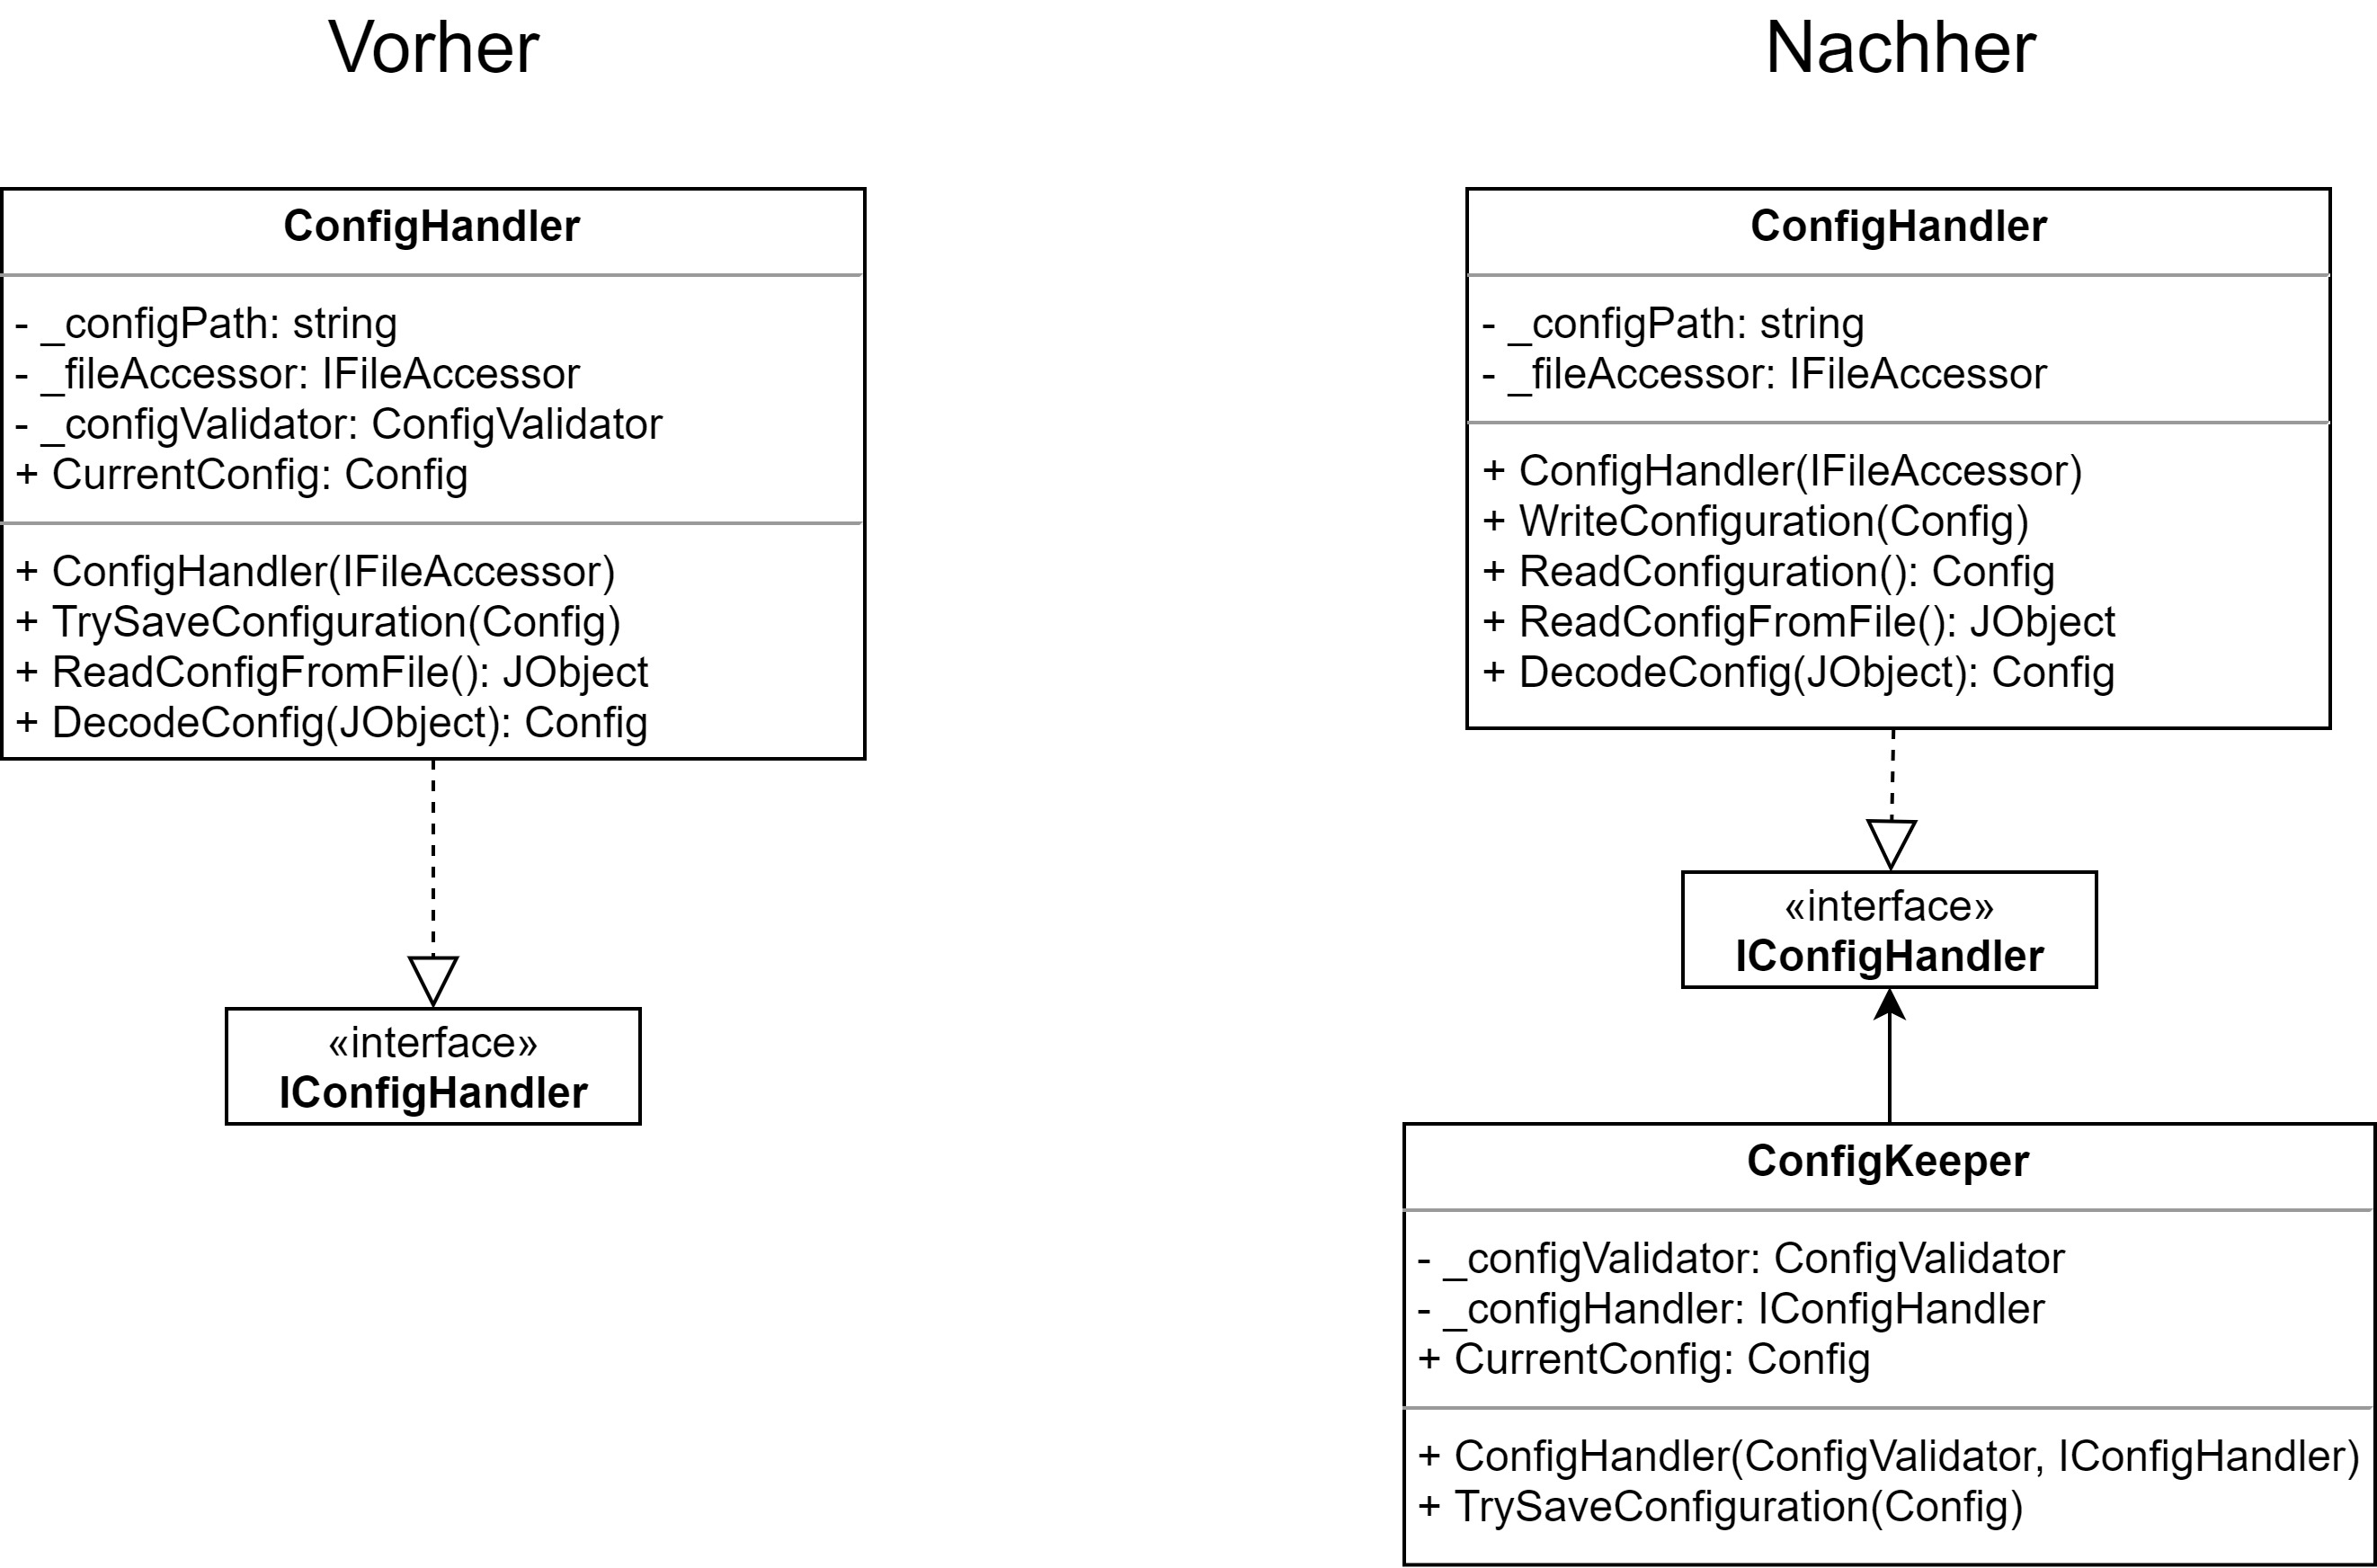
\includegraphics[width=0.8\textwidth]{Bilder/ConfigHandlerSRP}
\caption[Single Responsibility Principle: ConfigHandler Vorher - Nachher]{\label{fig:ConfigHandlerSRP} Single Responsibility Principle: ConfigHandler Vorher - Nachher}
\end{figure}
\subsubsection{Open/Closed Principle}
Das Open/Closed Principle beschreibt, dass Softwäre-Entitäten offen für Erweiterung aber geschlossen bezüglich Veränderung sein sollen. Dementsprechend soll bestehender Code nicht mehr geändert werden. Bei neuen bzw. geänderten Anforderungen wird der bestehende Code also nicht angepasst/geändert, sondern lediglich erweitert.\\

\noindent Bei unserer Anwendung identifiziert man eine mögliche Entwicklung mit Erweiterung klar bei der Validierung der Konfiguration, hier wird also das OCP verletzt. Gerade wenn sich diese in der Zukunft nochmals anpassen sollte, weil bspw. noch weitere Präferenzen des Nutzers/der Nutzerin erfasst werden sollen.
\begin{listing}[h]
\inputminted[linenos=true,frame=lines, breaklines, breakanywhere]{csharp}{Listings/ValidateInputsPre.cs}
\caption{Verletzung des Open/Closed-Principle im ConfigValidator}
\label{ConfigValidatorPre}
\end{listing}
In Listing \ref{ConfigValidatorPre} ist erkennbar, dass der Code zum Überprüfen angepasst werden müsste, falls eine neue Anforderung an die Konfiguration hinzugefügt wird. Daher wird der bisherige \texttt{ConfigValidator} umgeschrieben und hält nun eine \texttt{List<IValidationAspect>}. In dieser Liste sind alle Validierungs-Aspekte gespeichert gegen die die Eingabe getestet werden soll. Das Interface \texttt{IValidationAspect} definiert eine Methode \texttt{Validate(Config)}, welche validiert, ob die Regel eingehalten wurde. Sollte dies nicht der Fall sein, wird eine Exception geworfen. Nun muss im \texttt{ConfigValidator} lediglich über alle registrierten \texttt{IValidationAspects} iteriert werden und mit der übergebenen Config die \texttt{Validate}-Methode aufgerufen werden. Das Hinzufügen einer neuen Anforderung ist nun simpel über das Schreiben einer neuen Klasse möglich. Diese muss \texttt{IValidationAspect} implementieren und auf den \texttt{ConfigValidator} registriert werden. Der neue \texttt{ConfigValidator} und ein Beispiel für einen \texttt{IValidationAspect} ist in Listing \ref{ConfigValidatorPost} zu sehen. Hierbei ist zu beachten, dass bei negativem Testergebnis eine Exception geworfen (und kein false zurückgegeben) wird, um die genaue Fehlerursache dem Nutzer/der Nutzerin mitzuteilen. Wird keine Exception geworfen, ist mit der Konfiguration alles in Ordnung.\\

\begin{listing}[h]
\inputminted[linenos=true,frame=lines, breaklines, breakbytokenanywhere]{csharp}{Listings/ValidateInputsPost.cs}
\caption{Entwicklung mit Erweiterung für den ConfigValidator}
\label{ConfigValidatorPost}
\end{listing}

\noindent Ein Punkt an dem das OCP nicht erfüllt ist, ist der \texttt{WeatherInterpreter}. Sollten in Zukunft weitere Daten zur Interpretation des Wetters dazu kommen, so müsste der Code des \texttt{WeatherInterpreters} angepasst und verändert werden.
\subsubsection{Liskov Substitution Principle}
Das Liskov Substitution Principle sagt aus, dass Subtypen sich so wie ihr Basistyp verhalten müssen. Subtypen dürfen daher lediglich die Funktionalität ihres Basistyps erweitern, aber nicht einschränken.
Das Liskov Substitution Principle ist in unserer Anwendung erfüllt, da abgesehen von den verwendeten Interfaces keine Vererbung verwendet wird.
\subsubsection{Interface Segregation Principle}
Das Interface Segregation Principle sagt aus, dass Interfaces passgenau für die aufrufenden Clients sein muss. Das Interface darf also keine Details beinhalten, die der Client gar nicht benötigt.
Die Interfaces unserer Anwendung folgen diesem Prinzip.\\

\noindent Anhand des Interfaces \texttt{IFileAccessor} kann man die Entwicklung hin zum Erfüllen des Prinzips gut nachvollziehen, da das Interface \texttt{IFileAccessor} von zwei Klienten verwendet wird. Dabei benötigt einerseits der \texttt{ConfigHandler} den Zugriff auf Dateien (Lesen und Schreiben) und andererseits der \texttt{DownloadHelper} die Möglichkeit das Hintergrundbild zu speichern. Das Interface \texttt{IFileAccessor} umfasst daher sowohl das Lesen/Schreiben von Dateien als auch das Schreiben von Bildern. Dieses Interface wurde dementsprechend, um das Interface Segregation Principle zu erfüllen, in zwei Interfaces aufgeteilt. Einerseits das Interface \texttt{IImageWriter} und andererseits das (bereits bestehende) Interface \texttt{IFileAccessor}. Wie der Name schon sagt, kümmert sich das Interface \texttt{IImageWriter} um das Schreiben von Bildern und das Interface \texttt{IFileAccessor} mit dem Lesen und Schreiben von Dateien. In \href{https://github.com/Bronzila/WeatherWallpaper/commit/8db38466c2185e16ef90f71af485e00b57b09032}{\color{blue}diesem Commit} ist das Segmentieren dieser beiden Interfaces zu erkennen.
Generell haben einige Interfaces das ISP nicht erfüllt, allerdings war keins dieser Beispiele so eindringlich wie das Obere, da die meisten Interfaces nur ein aufrufenden Client hatten und auf diesen einzelnen Client nicht passgenau zugeschnitten waren. Mittlerweile wurden auch die Interfaces, die das Prinzip nicht erfüllt haben so umgeschrieben, dass sie es erfüllen.
\subsubsection{Dependency Inversion Principle}\label{sec:dependency_inversion}
Mit dem Dependency Inversion Principle wird versucht höhere Ebenen von niedrigeren Ebenen zu entkoppeln. Dabei gilt die Regel, dass Abstraktionen nicht von Details abhängen sollen, sondern Details von Abstraktionen abhängen sollten, da Abhängigkeiten auf konkrete Klassen stark koppeln. Sollte dieses Prinzip nicht erfüllt sein, so würden Änderungen in der niedrigeren Ebene Änderungen in der höheren Ebene hervorrufen. Eine Verletzung dieses Prinzips wird mithilfe der Dependency Injection aufgelöst. Dabei sind die Klassen der höheren und niedrigeren Ebene abhängig von einem Interface anstelle von  einer konkreten Klasse. Die Referenz auf die Instanz erhalten die Klassen der höheren Ebene dann meist im Konstruktor.\\

\noindent Die Verletzungen des Dependency Inversion Principle sind bei der Implementierung der Clean Architecture klar auffindbar. Sobald eine innere Schicht eine Abhängigkeit auf eine äußere Schicht hat, wird das Prinzip verletzt. In Kapitel \ref{CleanArchitectureVorher} sind diese Verletzungen nochmals kurz erläutert. Im Folgenden wird beispielhaft die Abhängigkeit vom damaligen \texttt{MainController} (mittlerweile umbenannt in \texttt{Refresher}) auf den \texttt{WeatherHandler} gezeigt. Hier wird das Prinzip verletzt, da sich der \texttt{Refresher} in der Application Code-Schicht befindet und der \texttt{WeatherHandler} in der Adapter-Schicht. Um dies zu beheben, wird das Interface \texttt{IWeatherHandler} eingesetzt. Der \texttt{Weather"-Handler} implementiert dieses und der \texttt{Refresher} hat nur noch die Abhängigkeit auf ein \texttt{I"-Wea"ther"-Hand"-ler}. Das tatsächliche Objekt erhält er dann im Konstruktor über Dependency Injection. In Abbildung \ref{DIP} ist dieser kleine Ausschnitt aus dem UML-Diagramm vereinfacht dargestellt und mit Vorher/Nachher betitelt.


\begin{figure}[ht]
\centering
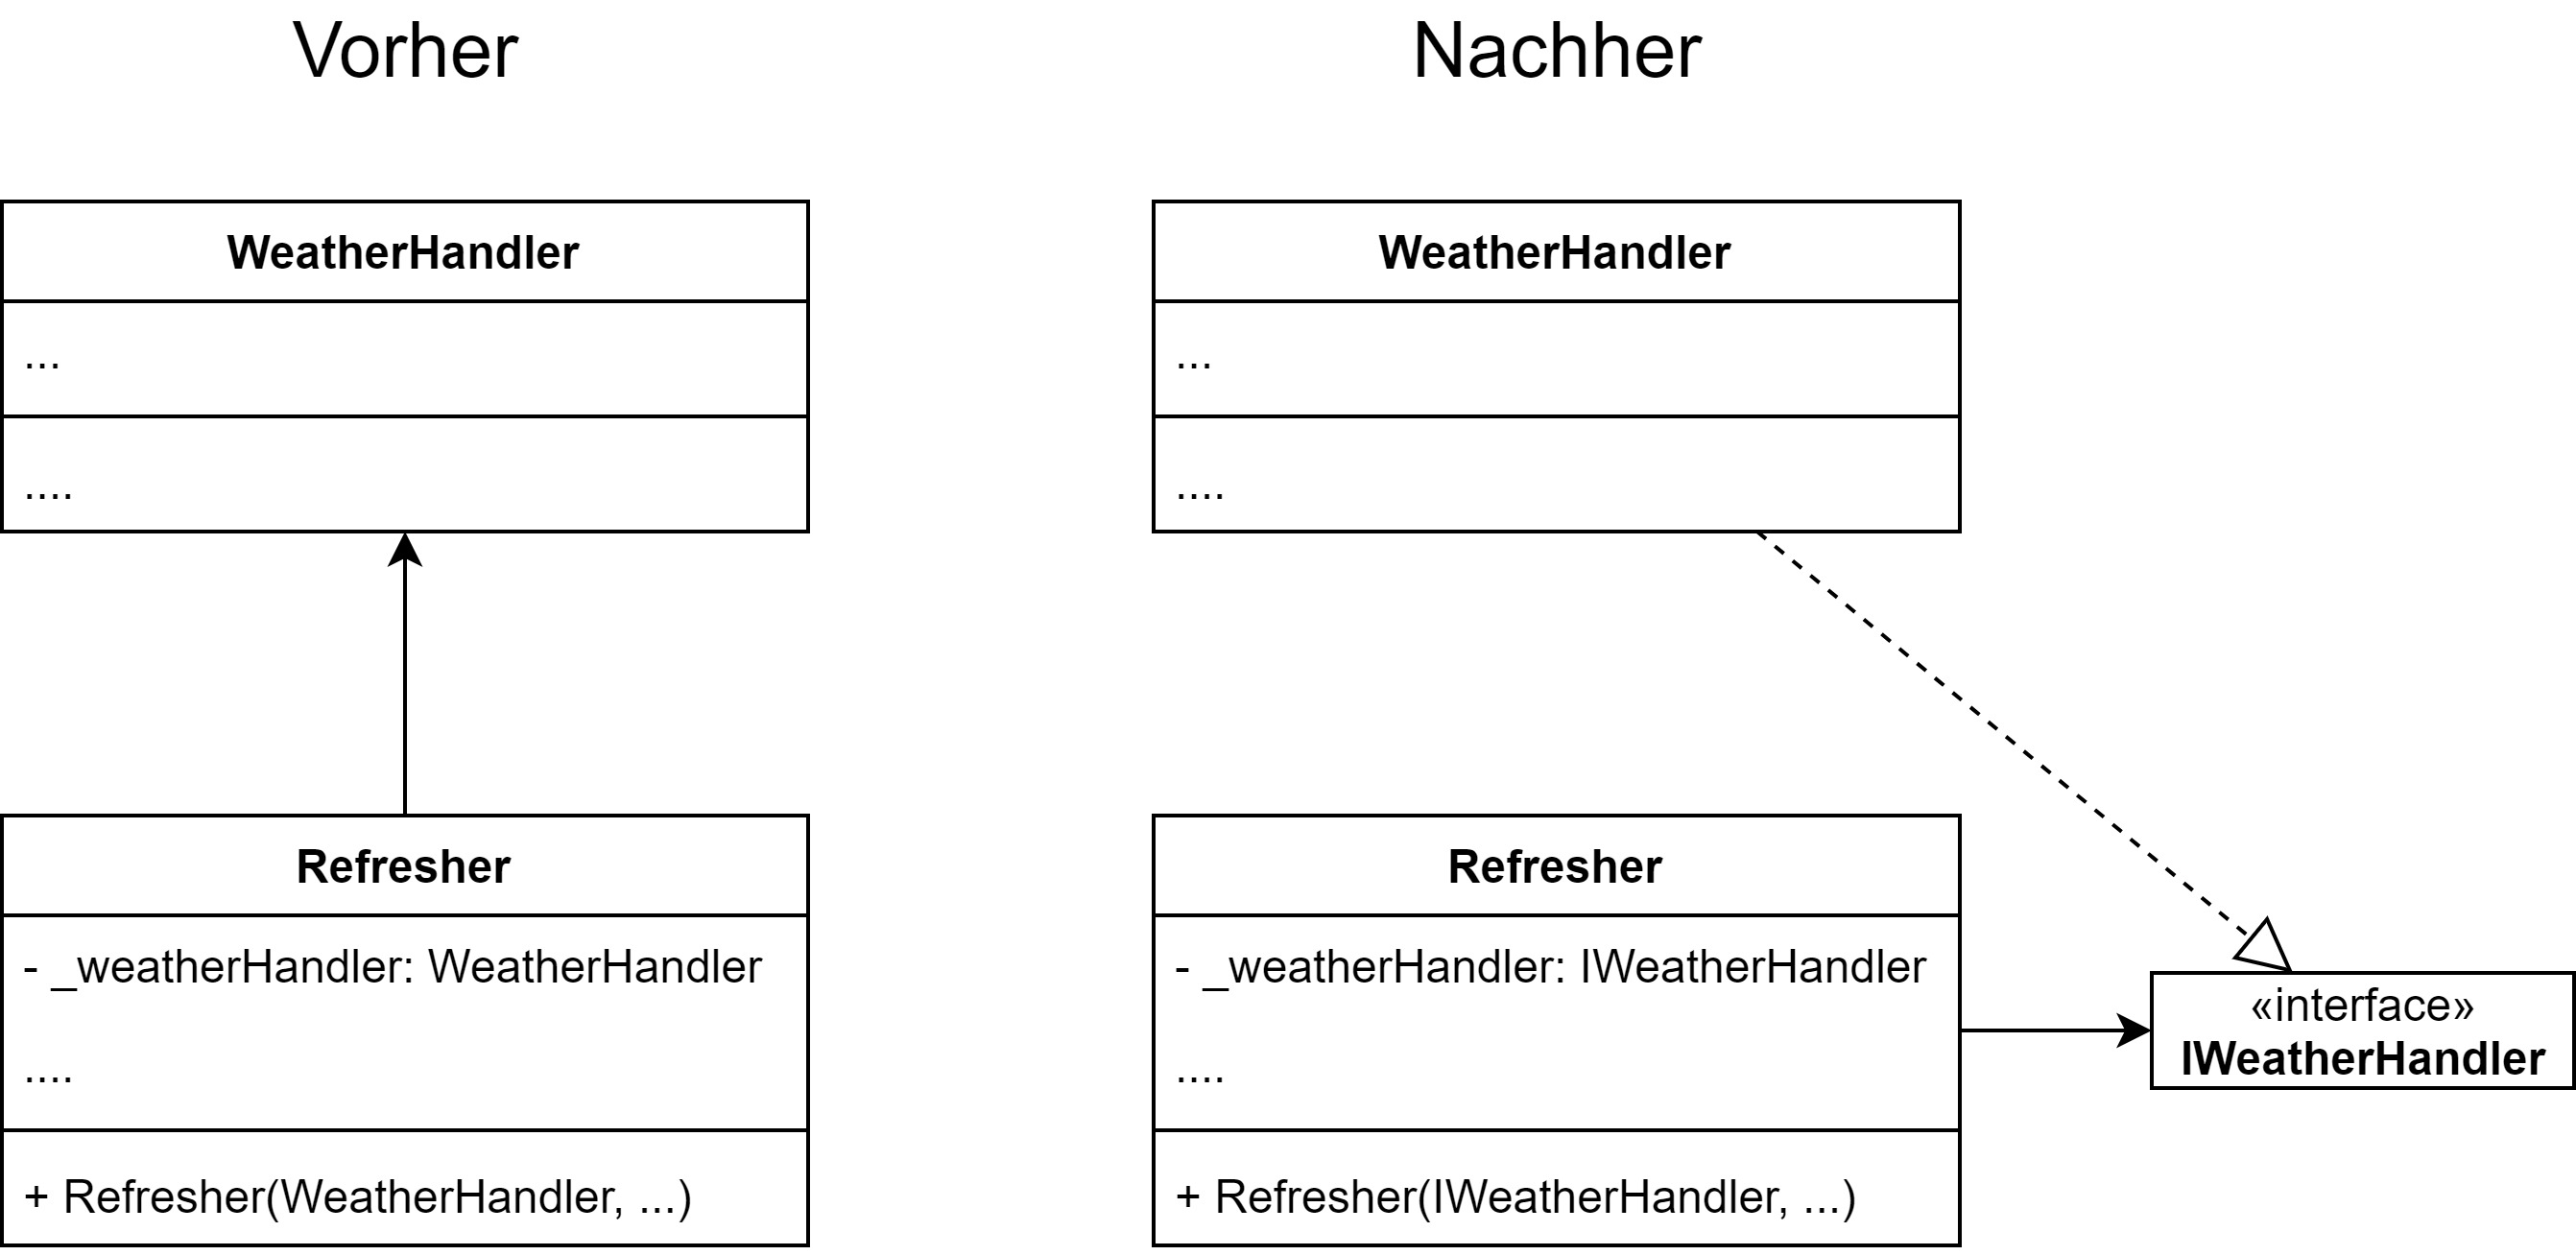
\includegraphics[width=0.8\textwidth]{Bilder/DIP}
\caption[Beispielhafte Verletzung und Verbesserung des DIP]{\label{DIP}Beispielhafte Verletzung und Verbesserung des DIP}
\end{figure}
\subsection{GRASP}
GRASP (General Responsibility Assignment Software Patterns/Principles) sind Stan"-dard"-lö"-sung"-en für typische Fragestellungen in der Software Entwicklung.
Diese wurden zum ersten mal von Craig Larman in seinem Buch \enquote{Applying UML and Patterns} aus dem Jahre 1995 vorgestellt.
Die ersten sechs dieser neun Prinzipien und deren Anwendung in unserem Programm werden im folgenden Verlauf erläutert.
%TODO
%\begin{itemize}
%	\item Low Coupling % geringe Koppelung zwischen den Klassen
%	\item High Cohesion % hoher Zusammenhalt innerhalb einer Klasse --> Prävention für SoC
%	\item Indirection % "andere arbeiten lassen" also Delegation
%	\item Polymorphism % Wo Funktionen geschrieben werden --> bei Änderungen in den Sub-Typen, ohne Änderung in der Oberklasse
%	\item Pure Fabrication % Trennung von Technologiewissen und Domänenwissen --> Auslagern einer Klasse als "Service" (in ddd), damit low coupling und high cohesion (und potentielle wiederverwendung) gegeben sind
%	\item Protected Variations % Schutz von Elementen vor Variation anderer Elemente --> "verstecken hinter gleicher Schnittstelle"
%\end{itemize}

\subsubsection{Low Coupling \& High Cohesion}
\label{sec:lc_hc}
Diese beiden Prinzipien sind essentielle Grundkonzepte bei GRASP.
\textit{Low Coupling} ist ein Maß über die Abhängigkeit einer Komponente zu ihrem Umfeld.
Das Prinzip ermöglicht vor allem eine höhere Anpassbarkeit der Komponente, ein einfacheres Verständnis über die Funktionsweise dieser und ein leichteres Testen aufgrund geringer Abhängigkeiten zu anderen Komponenten.
\textit{High Cohesion} hingegen gibt Auskunft über den Zusammenhalt innerhalb einer Komponente.
Es wird also gemessen, wie eng die Methoden und Attribute innerhalb einer Komponente (bspw. einer Klasse) zusammenarbeiten.
Dies reduziert hauptsächlich die Komplexität des Gesamtsystems, da Klassen sinnvoll strukturiert werden.
Beide bedingen sich gegenseitig: Code mit hoher Kohäsion besitzt oft eine geringe Kopplung.\\
\\
Die Klassen \texttt{WeatherHandler} und \texttt{ImageHandler} erhalten Informationen über die derzeitige Konfiguration bzw. über das aktuelle Wetter.
Sie sind dafür zuständig mithilfe der jeweiligen Information einen Query-String für die spätere API Abfrage zu erstellen.
Für das Zusammenstellen der zusätzlichen Abfrageattribute ist die jeweilige Funktion \texttt{BuildRouteString()} zuständig.
Beim \texttt{ImageHandler} beispielsweise wurde diese Funktion außerhalb der eigentlichen Klasse - in der Controller-Klasse \texttt{Refresher} - aufgerufen. Dabei wurde ein String mit zusätzlichen Abfrageparameter zusammengebaut und daraufhin die Funktion \texttt{GetImageData()} mit eben diesem String als Parameter aufgerufen. 
Im Codebeispiel \ref{lst:ImageHandler_old} ist die Klasse \texttt{ImageHandler} vereinfacht dargestellt. \\
\\
\begin{listing}[htb]
	\inputminted[linenos=true,frame=lines, breaklines, breakanywhere]{csharp}{Listings/ImageHandler_old.cs}
	\caption{Alte Implementierung des ImageHandlers mit hoher Kopplung und niedriger Kohäsion}
	\label{lst:ImageHandler_old}
\end{listing}

\noindent Dadurch besitzt die Klasse zwei direkte Kopplungen zur \texttt{Refresher} Klasse und gleichzeitig wird die Route-String Funktion nie in der eigenen Klasse aufgerufen.
Nach den genannten Prinzipien soll \texttt{BuildRouteString()} nicht mehr außerhalb, sondern aus der \texttt{GetImageData()} Funktion heraus aufgerufen werden. 
Da die Interpretation der aktuelle Wetterdaten zum Bau des Strings benötigt wird, muss diese der Funktion \texttt{GetImageData()} als Parameter übergeben werden an Stelle des fertigen Route-Strings.
Somit wird die Abhängigkeit der Klasse zum \texttt{Refresher} reduziert und gleichzeitig die Kohäsion erhöht.
Die neue Version wird in dem Beispiel \ref{lst:ImageHandler_new} gezeigt\footnote{Diese Änderungen wurden im Commit \url{https://github.com/Bronzila/WeatherWallpaper/commit/25e8c58a47945383746d8151ed4bfbed01b1d24c} durchgeführt.}.\\
\\
\begin{listing}[htb]
	\inputminted[linenos=true,frame=lines, breaklines, breakanywhere]{csharp}{Listings/ImageHandler_new.cs}
	\caption{Überarbeitung des ImageHandlers mit niedrigerer Kopplung und hoher Kohäsion}
	\label{lst:ImageHandler_new}
\end{listing}

\noindent Ähnliches wurden ebenfalls für die \texttt{WeatherHandler} Klasse mit der Funktion \texttt{Location"-As"-Route"-Attribute()} geändert.
Auch hier verringert sich die Abhängigkeit und die Kohäsion steigt.

\subsubsection{Indirection}
Unter \textit{Indirection} versteht man die zentrale Verwaltung von Aufgaben an einzelne Komponenten, wodurch untereinander keine direkte Kopplung bestehen muss.
Somit ist es ein Prinzip zur Code-Strukturierung und kann zu geringer Kopplung führen, da eine direkte Abhängigkeit der Klassen untereinander vermieden wird.
Gleichzeitig bietet diese Struktur trotzdem weiterhin gute Möglichkeiten Komponenten wiederzuverwenden.\\
\\
\noindent Bei unserem Programmentwurf soll ein Timer nach einem gewissen Intervall alle Aktionen zum Wechsel des Hintergrundbildes durchführen.
Da hierbei viele verschiedene Komponenten zusammenhängen, beispielsweise die Benutzeroberfläche, zwei unterschiedliche API-Abfragen und das Herunterladen eines Bildes, wäre das Projekt sehr schnell unübersichtlich und verschachtelt geworden.\\

\noindent Alle Klassen hätten somit untereinander eine Abhängigkeit und Wiederverwendbarkeit wäre nur eingeschränkt möglich.
Deshalb wurde die zentrale Klasse \texttt{Refresher} mit der Funktion \texttt{Refresh()} implementiert.
Diese kann vom Timer oder direkt aus der Benutzeroberfläche aufgerufen werden und \enquote{delegiert} die Arbeit an einzelne Klassen.
Funktionsaufrufe werden nacheinander ausgeführt und die benötigten Rückgabewerte als Parameter in die nächste Funktion übergeben.
Dadurch entsteht eine indirekte Abhängigkeit, wodurch alles übersichtlich bleibt.
% Ein ähnliches Prinzip findet sich beim Controller des Entwurfsmusters MVC wieder.
\subsubsection{Polymorphism}
\label{sec:polymorphism}
Ebenfalls zur Code-Strukturierung trägt das Prinzip des Polymorphismus bei.
Dadurch kann das Verhalten abhängig vom konkreten Typ jeweils geändert werden; Funktionen erhalten somit eine neue Implementierung.\\

\noindent Dies ist bei unserem Programm in der Klasse \texttt{ConfigValidator} deutlich zu erkennen.
Sie validiert die eingegebene Funktion, wobei mehrere Validierungsaspekte separat in Betracht gezogen werden.
Validierungsaspekte sind Implementierungen des Interfaces \texttt{IValidationAspect}, welches eine Funktion \texttt{Validate(Config)} besitzt.\\

\noindent Diese Aspekte können nun einzeln über die Funktion \texttt{Register(IValidationAspect)} zu einer Liste hinzugefügt werden. 
Über \texttt{ValidateInputs(Config)} wird die eingegebene Konfiguration anhand dieser Aspekte überprüft.
Dafür wird mit jedem Aspekt in der Liste die jeweilige Funktion \texttt{Validate(Config)} aufgerufen.
Da die Implementierungen dieser Funktion sich von Typ zu Typ unterscheiden, liegt hier, durch den polymorphen Funktionsaufruf, eine indirekte Konditionalstruktur, also Polymorphismus vor.
Im Listing \ref{lst:ConfigValidator} ist der Zusammenhang von \texttt{IValidationAspekt} und \texttt{ValidateInputs(Config)} deutlich gezeigt.


\subsubsection{Pure Fabrication}\label{sec:pureFabrication}
Um eine geringe Kopplung und gleichzeitig hohe Kohäsion erreichen zu können, trennt dieses Prinzip die Problemdomäne von der zugrundeliegenden Technologie.
Es entsteht also eine Klasse ohne jeglichen Bezug zum Problem, sie kann somit überall wiederverwendet werden - eine reine Service Klasse bei Domain-Driven-Design.
Daher beschreibt das Prinzip den Aufbau der Architektur im Einklang mit den anderen Prinzipien.\\
\\
Wie bereits in Kapitel \ref{sec:srp} beschrieben war die Klasse \texttt{ConfigHandler} bisher für die Verwaltung der Konfiguration des Nutzers sowie das Konvertieren zwischen C\#-Objekt und JSON zuständig. Durch das Trennen dieser beiden Use-Cases wurde nicht nur das SRP eingehalten, sondern auch die Pure Fabrication. Das Domänen-Wissen, also das Verwalten und Halten der aktuellen Konfiguration ist im \texttt{ConfigKeeper} hinterlegt und das Technologie-Wissen, also das parsen von JSON-Objekten ist im \texttt{ConfigHandler} vorhanden.\\
\\
Die Klasse \texttt{ConfigValidator} kümmert sich, wie in Kapitel \ref{sec:polymorphism} beschrieben um das Problem der Validierung einer Konfiguration.
Hierbei werden verschiedene Validierungsaspekte in Betracht gezogen; jeder Aspekt wird einzeln validiert.
Die Methode \texttt{ValidateInputs(Config)} befindet sich somit in der Technologie-Ebene, da hier nur über mehrere Validierungsaspekte iteriert wird.
Die einzelnen Aspekte enthalten das Domänen-Wissen, ob die Konfiguration für diesen Aspekt valide ist. 
Die Funktion \texttt{Validate(Config)} ist auf jeden Aspekt angepasst und bestätigt dessen Korrektheit.
Beide Funktionen sind in der Abbildung \ref{lst:ConfigValidator} dargestellt.

\begin{listing}[htb]
	\inputminted[linenos=true,frame=lines, breaklines, breakbytokenanywhere]{csharp}{Listings/ConfigValidator.cs}
	\caption{ConfigValidator als Technologiewissen und IsCorrectCity als Problemdomäne}
	\label{lst:ConfigValidator}
\end{listing}

%\begin{itemize}
	%\item \texttt{ConfigValidator} ist Pure fabrication und einzelne %\texttt{IValidationAspect}s sind domain Code 
%	\item \texttt{StartUpHelper} 		% Reine Dienstklasse
%	\begin{itemize}
%		\item \texttt{ImageHandler}
%		\item \texttt{WeatherHandler} 	% Kein wirklicher Code von der Problemdomäne
%		\item \texttt{ConfigHandler} 	% current config als "state" --> gehört er also wirklich rein? .. SRP?
%	\end{itemize}
%\end{itemize}

\subsubsection{Protected Variations}
Um Elemente bei der Kopplung mit variierenden Implementierungen zu schützen, soll laut diesem Prinzip über eine gemeinsame Schnittstelle zugegriffen werden.
Somit können Veränderungen eines Elementes keinen (unerwünschten) Einfluss auf andere Elemente haben.\\
\\
Bei der Clean Architecture ist über das Dependency Inversion Prinzip (siehe Kapitel \ref{sec:dependency_inversion}) geregelt, dass Ab"-häng"-ig"-kei"-ten von innen nach außen zu jeder Zeit über ein Interface umgekehrt werden können und somit der Dependency Rule entsprechen.
Dies ist ein generelles Beispiel von Protected Variations, da man somit die innere Schicht über eine gemeinsame Schnittstelle vor einer möglichen Änderung der äußeren Schicht schützt.\\
\\
Ein genaueres Beispiel ist das Interface \texttt{IAPICaller}, welches den Aufruf aus beispielsweise der Klasse \texttt{ImageHandler} (Adapter-Schicht) auf die Klasse \texttt{APICaller} (Plugin-Schicht) ermöglicht.
Es wird also dem \texttt{ImageHandler} sichergestellt, dass er über die Funktion \texttt{Get(string)} Daten über Bilder erhält.
Somit kann eine Änderung der jeweiligen Implementierung der Beschaffungsart keinerlei Schaden beim \texttt{ImageHandler} verursachen, da eine klare gemeinsame Schnittstelle mit gegebenen Parametertypen und Rückgabetypen genutzt wird. Er muss somit nicht angepasst werden, wenn eine beschriebene Änderung vorliegt.\\
\\
Ähnliches gilt auch für das Interface \texttt{IBackgroundChanger}.
Das Wechseln des Hintergrundbildes funktioniert auf verschiedenen Betriebssystemen (selbst bei verschiedenen Windowsversionen) unterschiedlich. 
Um diesen Änderungen standhalten zu können, bietet das Interface mit der \texttt{Set(string)} Funktion eine einheitliche Schnittstelle.
Die jeweilige Implementierung kann nun geändert werden, ohne dass eine Änderung in einer inneren Schicht notwendig ist.
% ist das nicht immer wenn man aus einer "inneren" Schicht in einer "äußere" eine Abhängig hat
%\begin{itemize}
%	\item \texttt{IBackgroundChanger} Das Wechseln des Hintergrundbildes funktioniert auf verschiedenen Betriebssystemen (verschiedener Windowsversionen) unterschiedlich. Um dieser Änderungen standzuhalten bietet das Interface eine einheitliche Schnittstelle
%	\item \texttt{IImageWriter} Selbes
%	\item \texttt{IFileAccessor} Selbes
%	\item \texttt{IAPICaller} Bei Änderung der Beschaffungsart der Wetter- bzw. Bild Daten 
%\end{itemize}
\subsection{DRY}
\label{sec:dry}
Das Prinzip \textit{Don't Repeat Yourself} zielt darauf ab, Code-Wiederholungen durch Normalisierung und Abstraktion zu eliminieren.
Es wird also darauf geachtet, dass Code nur an einer einzigen Stelle im System geschrieben und verwaltet wird.\\
\\
Bei WeatherWallpaper werden Anfragen an insgesamt zwei APIs versendet.
Hierfür wurde das Interface \texttt{IAPICaller} jeweils in den Klassen \texttt{ImageAPICaller} und \texttt{WeatherAPICaller} implementiert.
Beide Klassen waren allgemein sehr ähnlich und unterschieden sich hauptsächlich über den HTTPClient, welcher logischerweise unterschiedliche Basisadressen erhält um die jeweilige API zu erreichen.
Gleichzeitig sind statische Felder, wie z.B. der API-Key oder andere, fix ausgewählte Parameter unterschiedlich.
Beide Klassen verfügten über eine \texttt{Get()} Funktion, welche die variablen Parameter als String übergeben bekommen hat und die API Anfrage über den HTTPClient mit entsprechender Adresse ausführt.\\
\\
Aufgrund dieser Ähnlichkeit wurden beide Klassen als \texttt{APICaller} nach dem DRY-Prinzip zusammengefasst.
Diese Klasse  erhält im Konstruktor zusätzlich zum HTTPClienten eine Liste von Strings mit API-spezifischen Feldern.
Diese Felder werden nun im Konstruktor in gleicher Reihenfolge als String zusammengebaut und ersetzen somit die statischen Felder in der Klasse selbst\footnote{Diese Änderung wurden im Commit \url{https://github.com/Bronzila/WeatherWallpaper/commit/fb4546895d2241b8ea2391991f102bcd8f2fb685} durchgeführt.}.
\subsection{YAGNI}
Das Prinzip \textit{You ain't gonna need it - du wirst es nicht brauchen} besagt, dass Code nur hingeschrieben wird, wenn dieser auch wirklich nötig ist.
Ungenutzter Code muss nämlich zeitintensiv implementiert, getestet, dokumentiert und gewartet werden; er bringt also deutlichen Zusatzaufwand mit sich.
Daher versucht dieses Prinzip diesen sogenannten Annahme-Code zu minimieren, bzw. eliminieren.\\
\\
Ursprünglich war angedacht, dieses Projekt mit Hardware zu verknüpfen, an welcher dann etwa Temperatur oder Wetter allgemein angezeigt werden sollte.
Hierfür war im \texttt{APICaller} eine \texttt{Put()} Methode bereits vorgesehen, jedoch nicht implementiert. 
Diese wurde nach diesem Prinzip verabschiedet, damit eben kein Annahme-Code mehr verwaltet werden muss\footnote{Die Funktion wurde mit der ersten Umstrukturierung des APICallers im Commit \url{https://github.com/Bronzila/WeatherWallpaper/commit/d11c44ef92c85fed125288c195fb36ce595c660d} entfernt.}.
% PUT Methode beim APICaller zunächst hinzugefügt, da ursprünglich angedacht war, das Ganze mit Hardware zu verknüpfen
% Diese wurde jedoch entfernt, da wir uns auf die wirklich relevanten Use Cases konzentriert hatten --> You Aint Gonna Need It

	\clearpage
	\section{Unit Tests}
	% TODO
Insgesamt wurden 29 Unit-Test geschrieben.
\subsection{ATRIP}
\subsection{Mocks}
\subsection{Code Coverage}
\begin{itemize}
	\item $>=$ 10 Unit Tests
	\item ATRIP-Regeln
	\item Code Coverage
	\item Einsatz von Mocks
\end{itemize}

	\clearpage
	\section{Refactoring}
	% TODO
\begin{itemize}
	\item Code Smells identifizieren
	\item $>= 2$ Refactoring anwenden und begründen

\end{itemize}
	
	
	
	
	
\end{document}




%************************************************************%
%*********************End of document************************%
%************************************************************%

\footnote{\url{https://de.wikipedia.org/wiki/Alufolie}} 


Abbildung \ref{fig:allg_kennlinie}

\begin{figure}[tbt]
	\begin{center}
		\includegraphics[scale=0.45]{Grafiken/allg_kennlinie.png}
	\end{center}
	\caption{Kennlinie einer Halbleiterdiode \protect \footnotemark}
	\label{fig:allg_kennlinie}
\end{figure}
\footnotetext{FUSSNOTE}


Tabelle \ref{tab:cobalt}

\begin{table}[tbt]
	\caption{•}
	\begin{threeparttable}	%Scheme for footnotes in tables
		\begin{center}
			\begin{tabular}{c c c c}
				\toprule
				& keV & keV & keV \\
				\midrule
				a	& b	& c	& d \\
				a	& b	& c	& d \\
				a	& b	& c	& d \\
				a	& b	& c	& d \\ %direkt hinter jeweiligen Wert /tnote{1}
				\bottomrule
			\end{tabular}
		\end{center}
		\begin{tablenotes}\footnotesize 
			\item[1]{Quelle: http://www.thinksrs.com/downloads/PDFs/ApplicationNotes/IG1BAgasapp.pdf}
		\end{tablenotes}
	\end{threeparttable}
	\label{tab:cobalt}
\end{table}